\documentclass[../sparc.tex]{subfiles}
\graphicspath{{\subfix{../images/}}}
\begin{document}

\newpage
%%%%%%%%%%%%%%%%%%%%%%%%%%%%%%%%%%%%%%%%%%%%%%%%%%%%%%%%%%%%%%%%%%%%%%%%%%%%%%%%
\section{Создание игрового движка}
\index{Разработка игр!Игровой движок}

%%%%%%%%%%%%%%%%%%%%%%%%%%%%%%%%%%%%%%%%%%%%%%%%%%%%%%%%%%%%%%%%%%%%%%%%%%%%%%%%
\subsection{Что такое ``Игровой движок''?}
В разработке игр со временем у программистов собирается набор необходимых
процедур и типов данных (структур), которые были созданы специально для
упрощения работы над игрой.  Используя эти специализированные инструменты, мы
можем быстро развивать логику игры, без необходимости снова и снова обращаться к
низкоуровневым механизмам, вроде рисования пикселей на экране, алгоритами
движения объектов по карте и т.п.

Когда команда разработчиков сталкивается с необходимостью создавать новую версию
игры, или даже совершенно новую игру -- часто оказывается, что базовые задачи уже
были решены в предыдущей игре.  Не удивительно, ведь работа с игровой картой,
отрисовка текстур, воспроизведение звуков и просчитываение физики существуют во
многих играх.  Зачем же повторять сделанную работу, если мы можем обратиться к
уже созданным процедурам и структурам данных?

Таким образом, мы приходим к тому, чтобы создать свой \emph{игровой движок} --
библиотеку функций и типов, созданных специально для разработки игр.  Даже если
мы будем применять наш движок только для одной игры, это даст нам преимущество в
плане модульности и упорядоченности нашего кода.

На базовом уровне, разработка игрового движка сводится к выносу наших типов
данных и процедур в отдельные файлы.  Это уже следующий уровень модульности --
сначала мы делили логику на процедуры, теперь будем группировать эти процедуры
по отдельным файлам, согласно их назначанию.

Чтобы понять, как правильно сделать это разделение нашего проекта на файлы, мы
должны разобраться с тем, что из себя представляет процесс сборки нашего проекта
в единый исполняемый файл.

%%%%%%%%%%%%%%%%%%%%%%%%%%%%%%%%%%%%%%%%%%%%%%%%%%%%%%%%%%%%%%%%%%%%%%%%%%%%%%%%
\subsection{Этапы сборки приложения}

До этого мы рассматривали сборку приложения, как некий неделимый процесс --
нажимаем на кнопку загрузки в интерфейсе Arduino IDE, и вот уже компьютер делает
какие-то действия с кодом нашего проекта, затем загружает программу в Arduino и
наконец мы получаем долгожданный мигающий светодиод.  Но не всё так просто, как
кажется на первый взгляд.

Конечно мы уже сталкивались с ситуациями, когда проект не собирался из-за
синтаксических ошибок в нашем коде -- забытые скобки и точки с запятыми дают о
себе знать уже на ранних этапах сборки.  В этом случае мы могли видеть в Arduino
IDE сообщения (порой, пугающие начинающих программистов) об ошибках.  Теперь
пришло время приподнять занавес тайны над процессом компиляции и посмотреть
внутрь.

В самом начале компьютер начинает работать с тем исходным кодом, который был
нами написан.  Важно понимать, что компьютер (точнее, его процессор) не понимает
напрямую наш язык программирования, и требуется специальный ``переводчик'' с
промежуточного языка (то есть, языка программирования) на низкоуровневые
машинные команды.  Однако это -- достаточно сложный процесс, который может быть
разбит на несколько основных этапов, как показано на
рис. \ref{fig:build-process}.

\figureBuildSteps{ru}

\subsubsection{Препроцессор}

Первым делом, исходный код (файл \texttt{main.ino}) обрабатывается
\emph{препроцессором} -- специальной программой.  На этом этапе из исходного кода
удаляются комментарии и обрабатываются \emph{директивы препроцессора} (также
называемые иногда \emph{командами препроцессора}.)  В языках C/C++ язык
пропроцессора является отдельным языком программирования, с достаточно
примитивным набором команд, который описывает операции, которые препроцессор
должен сделать с исходным кодом.

По своей сути, препроцессор оперирует тремя базовыми инструментами: удаление
кода, копирование и вставка.

Например, как мы уже говорили выше, комментарии (все строчки, которые начинаются
с двух прямых слэшей, или строчки. насположенные между \mintinline{cpp}{/*
  ... */}) удаляются и не проходят на дальнейшие этапы сборки.

Другими популярными директивами препроцессора, которые мы можем встретить,
являются команды \mintinline{cpp}{#include} и \mintinline{cpp}{#define}.

Команда \mintinline{cpp}{#define} (``define'' в переводе с английского означает
``определить'') обычно используется в таком ключе:

\begin{listing}[H]
  \begin{minted}[highlightlines={1, 8, 10}]{cpp}
    #define DELAY_TIME 100
    void setup() {
      pinMode(2, OUTPUT);
    }

    void loop() {
      digitalWrite(2, HIGH);
      delay(DELAY_TIME);
      digitalWrite(2, LOW);
      delay(DELAY_TIME);
    }
  \end{minted}
  \label{listing:preprocessor-define-example-1}
  \caption{Пример использования директивы препроцессора для задания константы.}
\end{listing}

В листинге \ref{listing:preprocessor-define-example-1} мы видим пример
использования \mintinline{cpp}{#define} для задания именованной константы
\mintinline{cpp}{DELAY_TIME}, определяющей время задержки между включением и
выключением светодиода.  В процедуре \mintinline{cpp}{loop} данная константа
подставляется в качестве значения задержки при вызове процедуры
\mintinline{cpp}{delay}.

Когда препроцессор встречает константу, определённую ранее через
\mintinline{cpp}{#define}, то он заменяет имя константы на фактическое её
значение.  Тут важно понимать, что препроцессор не делает почти никаких проверок
о корректности результата подстановки значения константы.  Таким образом, в
результате неправильного задания константы препроцессор подставить её значение
везде в коде, где константа упоминается, но на более поздних этапах сборки
произойдёт ошибка.

Кроме этого, мы можем видеть на первой строчке в листинге
\ref{listing:preprocessor-define-example-1}, что при объявлении подобной константы
мы не используем уже привычные нам типы данных, и даже не ставим в конце
вездесущую точку с запятой; более того, завершение строчки с
\mintinline{cpp}{#define} точкой с запятой приведёт впоследствии к ошибке.

Возникает вопрос: стоит ли использовать \mintinline{cpp}{#define}, когда у нас
есть ключевое слово \mintinline{cpp}{const}?  Ведь с тем же успехом мы могли бы
написать:

\begin{listing}[H]
  \begin{minted}[highlightlines={1}]{cpp}
    const int DELAY_TIME = 100;
    void setup() {
      pinMode(2, OUTPUT);
    }

    void loop() {
      digitalWrite(2, HIGH);
      delay(DELAY_TIME);
      digitalWrite(2, LOW);
      delay(DELAY_TIME);
    }
  \end{minted}
  \label{listing:preprocessor-define-example-2}
  \caption{Пример задания обычной константы.}
\end{listing}

Действительно, запись, показанная в листинге
\ref{listing:preprocessor-define-example-2} имеет много преимуществ перед
листингом \ref{listing:preprocessor-define-example-1}, где мы использовали
\mintinline{cpp}{#define}.  Например, заданная нами через
\mintinline{cpp}{const} константа имеет типизацию (тип данных
\mintinline{cpp}{int}), и при сборке подобного кода происходят все необходимые
проверки корректности синтаксиса (в отличии от \mintinline{cpp}{#define}.)  По
этой причине в большинстве случаев использование обычных констант
предпочтительнее, чем использование \mintinline{cpp}{#define}.

Но не стоит сразу списывать использование директив препроцессора со счетов --
ведь существуют случаи, когда использование препроцессора допустимо, и даже
необходимо.  Дело в том, что препроцессор выполняет операции именно над исходным
кодом программы, и таким в дальнейшую компиляцию попадает уже обработанный код.
Если мы посмотрим на промежуточное состояние нашего кода на C/C++ после работы
препроцессора, то не увидим там упоминания \mintinline{cpp}{DELAY_TIME},
заданного через \mintinline{cpp}{#define} -- вместо этого, на тех местах, где мы
на данную константу ссылались, будет уже стоять её значение (100).

Другой полезной для нас директивой проепроцессора является
\mintinline{cpp}{#include} -- данная директива инструктирует препроцессор
скопировать и вставить на её место содержимое того файла, на который она
ссылается.  Мы рассмотрим подробнее данную директиву в разделе
\ref{subsection:multi-file-applications}.

\subsubsection{Транслятор}

После препроцессора в работу вступает \emph{транслятор} -- его задачей является
преобразование высокоуровневого языка программирования (C/C++) в низкоуровневый
\emph{язык ассемблера}.  На данном этапе выявляются \emph{синтаксические
ошибки}, вроде пропущенных скобок и точек с запятыми, ссылок на несуществующие
переменные и т.п.

Получившийся код всё ещё может быть относительно легко прочитан (и даже изменён)
человеком, но он уже написан на гораздо более ``примитивном'' уровне.  После
этого, до машинного (двоичного) кода остаётся один шаг.

Код на ассемблере уже сильно зависим от процессора, под который идёт сборка -- у
разных процессоров может быть разный набор команд.  Говорят, что такой код
\emph{платформо-зависимый}.

\subsubsection{Ассемблер}

Далее в работу вступает программа-ассемблер.  Данная программа берёт код на
языке ассемблера и транслирует его в машинные команды -- непосредственно
низкоуровневые команды процессора, под который идёт сборка.

Результатом работы ассемблера является \emph{объектный файл} -- по сути, это файл
с машинным кодом.  Данный файл ещё не является \emph{исполняемым}, хотя внутри
него уже команды, которые процессор может прочитать и выполнить.

\subsubsection{Линковщик}

В конце исполняемый файл приложения собирается из нескольких ``кусочков'' --
объектных файлов приложения и сторонних библиотек.  Эту ``склейку'' паззла
проводит программа, называемая \emph{линковщиком} (или, буквально,
``связывателем''.)

В случае с Arduino, получившийся двоичный файл загружается на плату для
исполнения.

%%%%%%%%%%%%%%%%%%%%%%%%%%%%%%%%%%%%%%%%%%%%%%%%%%%%%%%%%%%%%%%%%%%%%%%%%%%%%%%%
\subsection{Разделение проекта на файлы}
\label{subsection:multi-file-applications}

В предыдущем разделе, где мы говорили про этапы сборки приложения, упоминалась
директива препроцессора \mintinline{cpp}{#include}.  Для изучения практического
применения \mintinline{cpp}{#include} разберём простой пример.  Допустим, мы
хотим вынести всё, что связано с игровыми звуками и музыкой, в отдельный файл --
``разгрузив'' таким образом основной файл с кодом нашего проекта.

В Arduino IDE нам доступно три основных вида файлов -- перечислим их расширения,
с кратким описанием назначения каждого вида файлов:
\begin{itemize}
\item \texttt{.ino} -- файлы с исходным кодом Arduino IDE.  Здесь мы можем писать
  всё то же, что мы до этого момента писали в главном (и единственном) файле
  нашего проекта.
\item \texttt{.h} -- так называемые \emph{заголовочные файлы}.  Их основное
  предназначение -- это хранение \emph{заголовков процедур} и помощь компилятору
  в связывании разрозненных файлов в один исполняемый файл.
\item \texttt{.с}, \texttt{.cpp} -- файлы с исходным кодом на языках C и C++. В
  целом, стандартное расшение файлов с исходным кодом этих языков, однако мы
  должны понимать, что в таких файлах изначально не доступны процедуры,
  специфичные для платформы Arduino (например, \mintinline{cpp}{digitalWrite},
  \mintinline{cpp}{pinMode}, \mintinline{cpp}{delay} и другие.)  Но мы можем
  подключить заголовочный файл \texttt{Arduino.h} через директиву
  \mintinline{cpp}{#include}, чтобы процедуры Arduino стали доступны в файлах
  ``.c'' и ``.cpp'' -- как делать включение файлов, будет рассказано далее.
\end{itemize}

Из всех перечисленных типов в дальнейшем мы будем использовать только
\texttt{.ino} и \texttt{.h}.

Первым делом в отдельный файл логично вынести процедуру
\mintinline{cpp}{play_tone}.  В терминологии Arduino IDE, файлы называются
\emph{``вкладками''}, и создать такую вкладку можно через специальное меню.

\begin{figure}[ht]
  \centering
  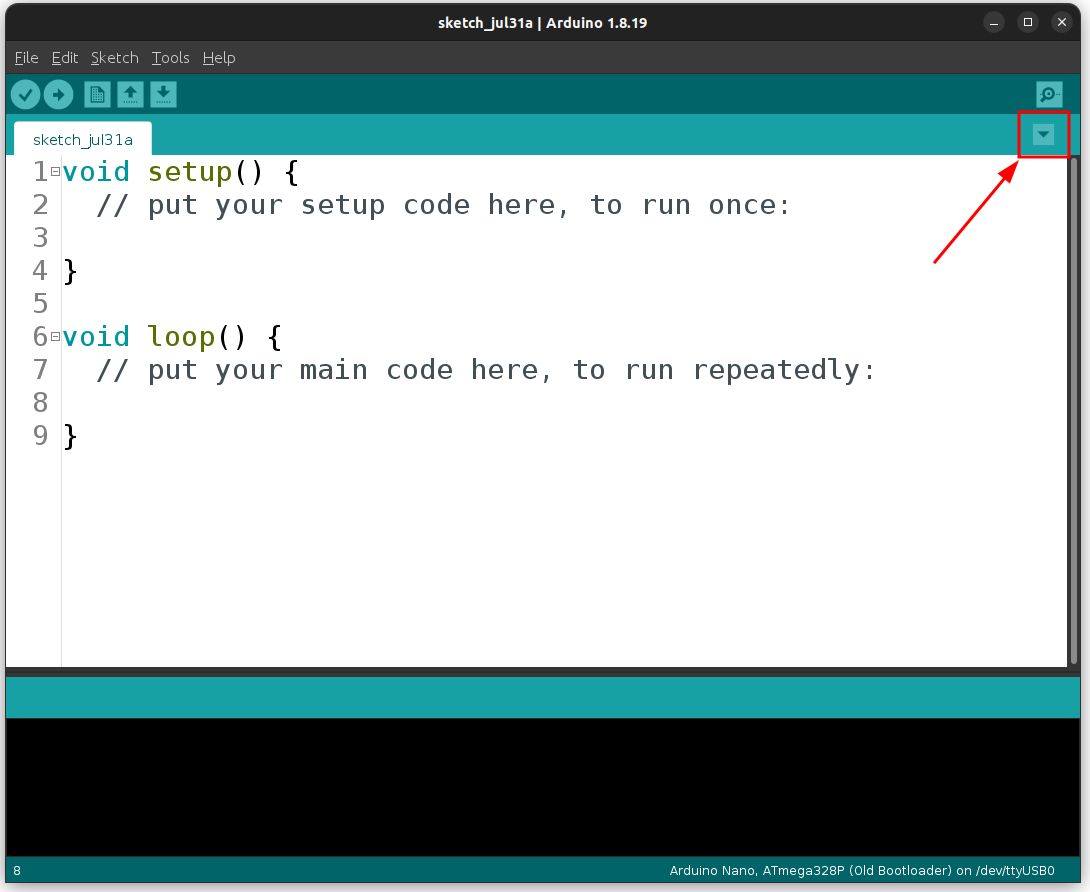
\includegraphics[width=10cm]{arduino-ide-tab-menu-button}
  \caption{Кнопка для управления ``вкладками'' (файлами) проекта в Arduino IDE.}
  \label{fig:arduino-ide-tab-menu-button}
\end{figure}

Мы будем использовать термин ``файл'' вместо ``владка'', когда будем ссылаться
на файлы проекта -- так как этот термин более стандартный с точки зрения
программирования.  С другой стороны, когда мы будем говорить про элементы
графического интерфейса Arduino IDE, отображающие файлы проекта -- мы будем
использовать термин ``вкладка'', так как это отражает способ их отображения в
интерфейсе редактора.

На рис. \ref{fig:arduino-ide-tab-menu-button} показана кнопка вызова меню работы
с вкладками в Arduino IDE версии 1.8.  Содержимое меню включает в себя следующие
пункты:

\begin{itemize}
\item ``New Tab'' (``Новая вкладка'') -- создание нового файла (``вкладки'') в
  текущем проекте.
\item ``Rename'' (``Переименовать'') -- переименовать текущую выбранную владку.
\item ``Delete'' (``Удалить'') -- удалить текущую выбранную вкладку.
\item ``Previous Tab'' (``Предыдущая вкладка'') -- переключиться на предыдущую
  вкладку проекта.
\item ``Next Tab'' (``Следующая вкладка'') -- переключиться на следующую вкладку
  проекта.
\item Название текущей вкладки.
\end{itemize}

Если нажать на ``New Tab'' (``Новая вкладка''), то в нижней части окна появится
поле для ввода имени новой вкладки, как показано на
рис. \ref{fig:arduino-ide-tab-name}.

\begin{figure}[h]
  \centering
  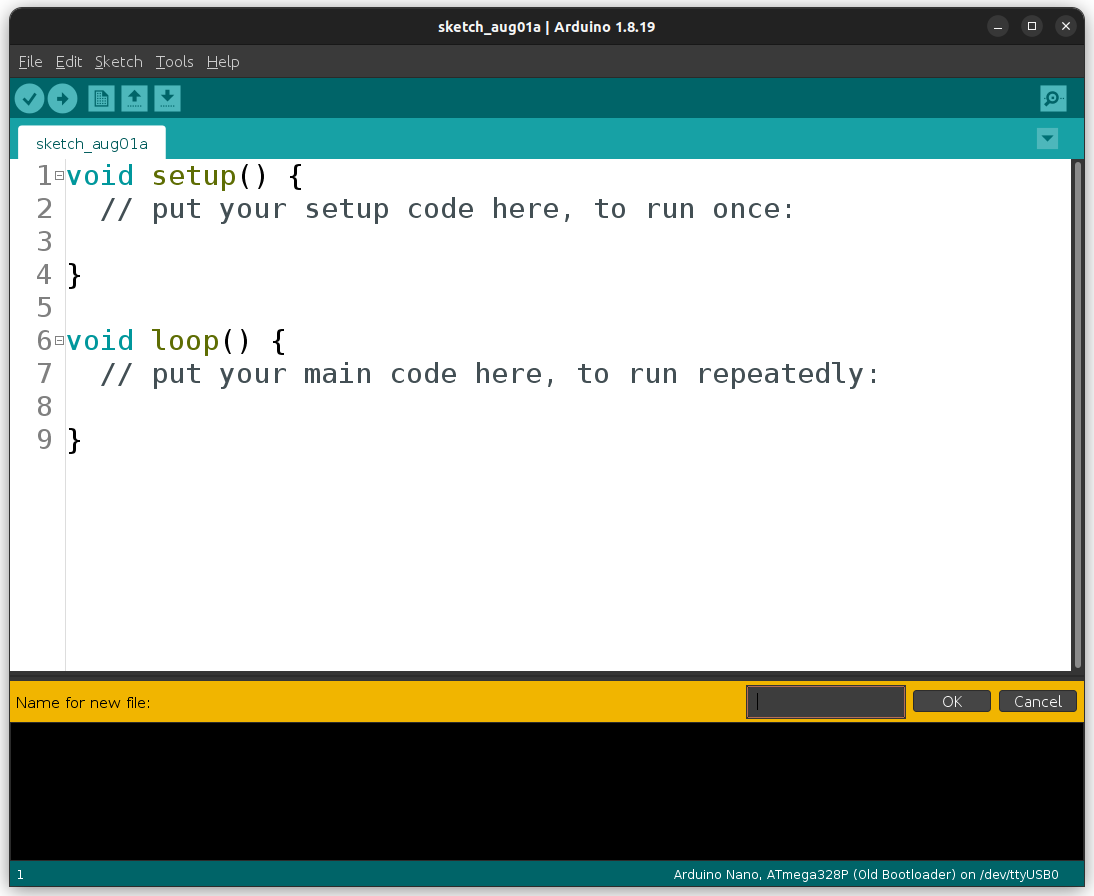
\includegraphics[width=10cm]{arduino-ide-tab-name}
  \caption{Поле для ввода названия нового файла в Arduino IDE.}
  \label{fig:arduino-ide-tab-name}
\end{figure}

Создадим файл с именем ``sound.ino'', вписав его в поле и нажав кнопку ``Ok''.
Важно писать имя файла с расширением, так как, строго говоря, расширение
является частью имени файла.  Результат создания нового файла показан на
рис. \ref{fig:arduino-ide-tab-sound-ino}.  Все ``.ino''-файлы автоматически
создаются в корне каталога проекта -- это позволяет Arduino IDE самостоятельно
находить все файлы, которые относятся к проекту, при сборке.

Файлы в проект можно также добавить вручную, разместив (или создав) их в корне
проекта, однако при этом потребуется перезапуск Arduino IDE для того, чтобы они
появились в виде ``вкладок'' в редакторе.

\begin{figure}[h]
  \centering
  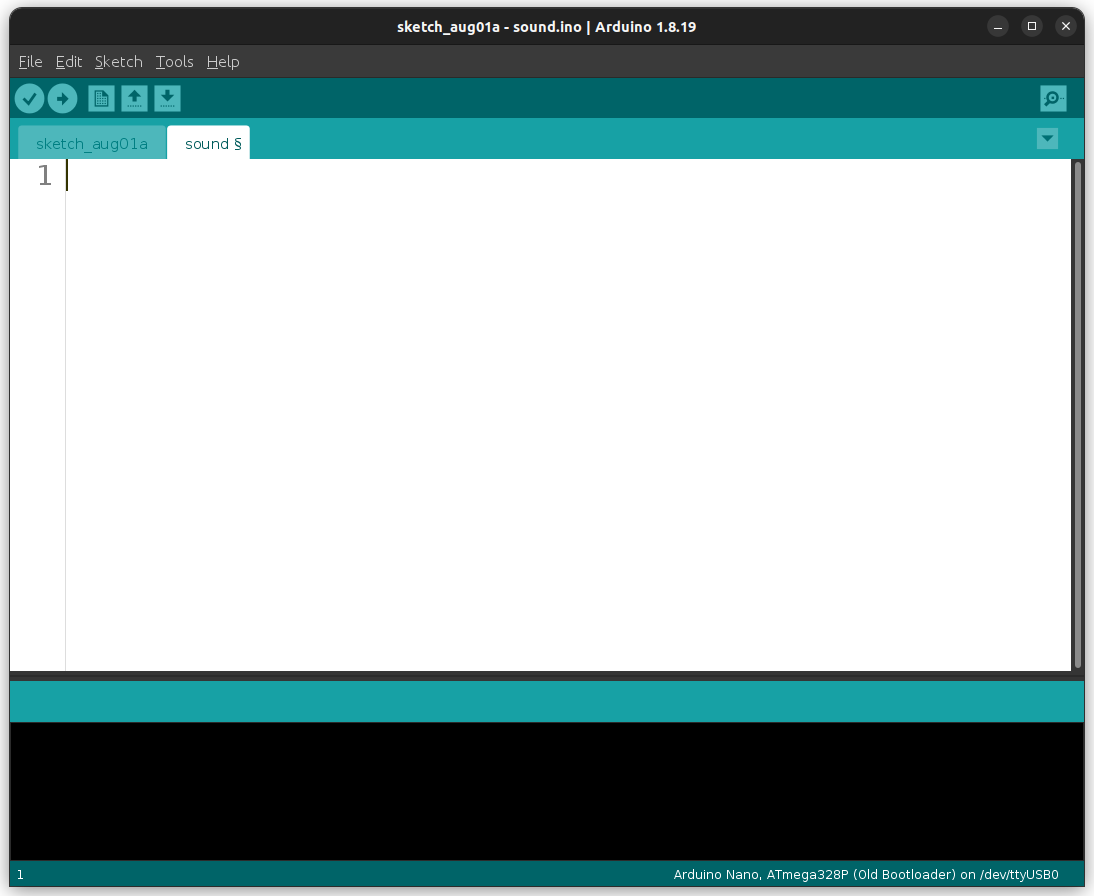
\includegraphics[width=10cm]{arduino-ide-tab-sound-ino}
  \caption{Результат создания файла с именем ``sound.ino'' в Arduino IDE.}
  \label{fig:arduino-ide-tab-sound-ino}
\end{figure}

В верхней части окна появится вкладка с названием ``sound'' -- для файлов с
раширением ``.ino'', данное расширение не отображается в названии вкладки.

Разместим процедуру \mintinline{cpp}{play_tone} в новом файле, как показано на
рис. \ref{fig:arduino-ide-tab-play-tone}.  Справа от названия вкладки можно
заментить значок параграфа (``\textsection'') -- это означает, что данный файл изменён и не
сохранён.  Если мы сохраним изменения в файле, данный значок пропадёт.

\begin{figure}[h]
  \centering
  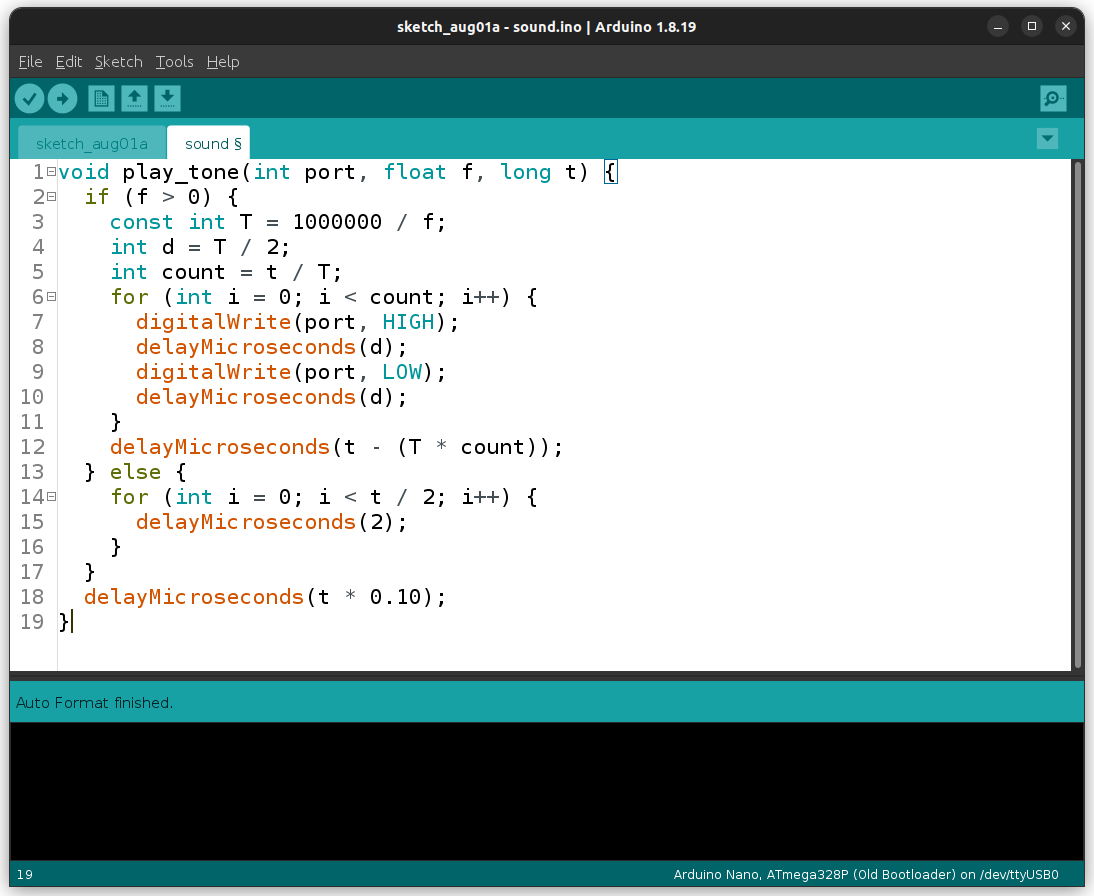
\includegraphics[width=10cm]{arduino-ide-tab-play-tone}
  \caption{Исходный код процедуры \mintinline{cpp}{play_tone} в файле ``sound.ino''.}
  \label{fig:arduino-ide-tab-play-tone}
\end{figure}

После того, как мы сохранили файл ``sound.ino'', можно вернуться на главый файл
(в нашем случае, он называется ``sketch\_aug01a.ino'', и вызывать оттуда
процедуру \mintinline{cpp}{play_tone}, как показано на
рис. \ref{fig:arduino-ide-tab-play-tone-call}.

\begin{figure}[h]
  \centering
  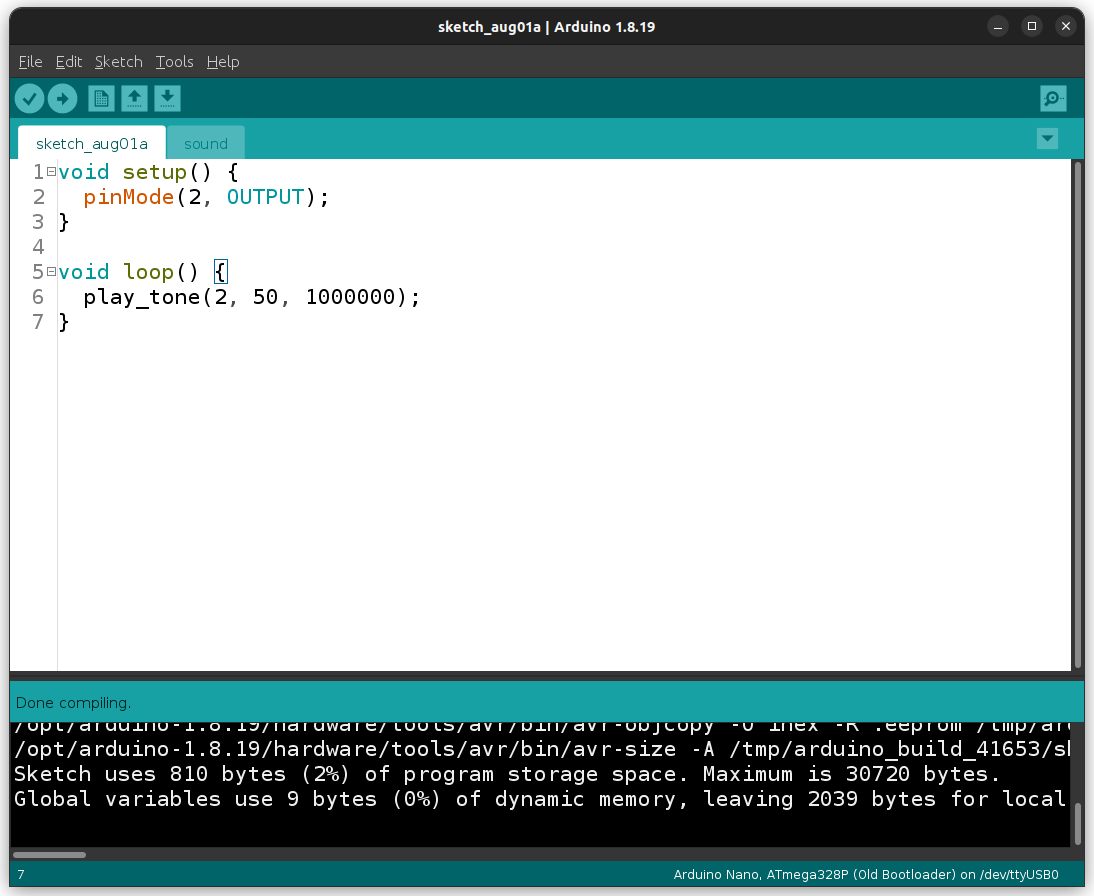
\includegraphics[width=10cm]{arduino-ide-tab-play-tone-call}
  \caption{Вызов процедуры \mintinline{cpp}{play_tone}, описанной в файле
    ``sound.ino''.}
  \label{fig:arduino-ide-tab-play-tone-call}
\end{figure}

На данном этапе проект должен уже успешно собираться и работать -- то есть,
компьютер смог собрать из двух файлов рабочий исполняемый файл.

\figureBuildStepsMultipleFiles{ru}

На рис. \ref{fig:build-process-for-two-files} показан процесс сборки приложения
из двух файлов с исходным кодом.  Мы видим, что каждый из файлов проходит
одинаковый путь от ``.ino'' до ``.o'', и затем линковщик ``склеивает'' эти два
файла воедино, создавая исполяемый файл.

Тем не менее, правильное деление проекта на несколько файлов требует наличие ещё
одного компонента -- так называемого \emph{заголовочного файла}, который обычно
имеет расширение ``.h''.  Этот файл будет парным для ``sound.ino'', и
следовательно логичным будет назвать его схожим образом -- а именно ``sound.h''.
На самом деле, совпадение имён файлов до расширения здесь не играет большой роли
-- мы дали им похожие имена, чтобы сделать структуру проекта более логичной и
понятной.

В чём же назначение заголовочного файла?  В первую очередь, заголовочные файлы
хранят \emph{заголовки процедур}.  Заголовком процедуры называется та часть её
объявления, которая включает возвращаемый тип, имя и параметры, без собственно
тела процедуры.  Для \mintinline{cpp}{play_tone} заголовок будет выглядеть, как
показано в листинге \ref{listing:game-dev-engine-procedure-header}.

\begin{listing}[H]
  \begin{minted}{cpp}
    void play_tone(int port, float f, long t);
  \end{minted}
  \label{listing:game-dev-engine-procedure-header}
  \caption{Заголовок процедуры.}
\end{listing}

Данный заголовок процедуры необходимо поместить в заголовочный файл ``sound.h'',
как показано на рис. \ref{fig:arduino-ide-tab-sound-header}.

\begin{figure}[h]
  \centering
  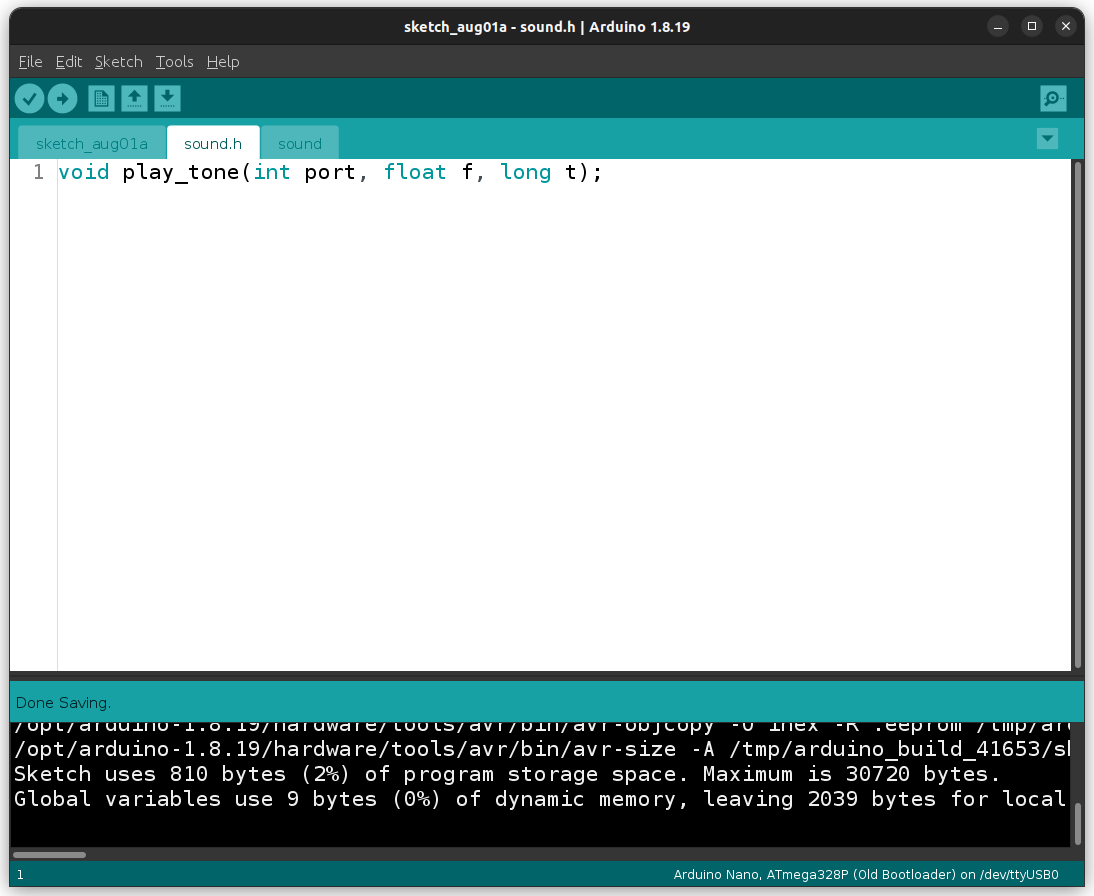
\includegraphics[width=10cm]{arduino-ide-tab-sound-header}
  \caption{Заголовочный файл ``sound.h'' с заголовком процедуры
    \mintinline{cpp}{play_tone}.}
  \label{fig:arduino-ide-tab-sound-header}
\end{figure}

Заголовочный файл необходимо \emph{включить} в тот файл с исходным кодом, где мы
будем ссылаться на процедуру \mintinline{cpp}{play_tone}, как показано в
листинге \ref{listing:game-dev-engine-procedure-header-include}.  Включение
файла производится с помощью директивы препроцессора \mintinline{cpp}{#include}
(в переводе с английского ``include'' означает ``включить''.)  В нашем случае,
включение необходимо сделать в основном файле нашего приложения
(``sketch\_aug01a.ino''.)

\begin{listing}[H]
  \begin{minted}[highlightlines={1}]{cpp}
    #include "sound.h"

    void setup() {
      pinMode(2, OUTPUT);
    }

    void loop() {
      play_tone(2, 50, 1000000);
    }
  \end{minted}
  \label{listing:game-dev-engine-procedure-header-include}
  \caption{Пример включения заголовочного файла ``sound.h'' с помощью директивы
    препроцессора.}
\end{listing}

Наличие заголовочного файла в нашей ситуации не обязательно, но оно помогает
компилятору выявлять ошибки вызова процедуры \mintinline{cpp}{play_tone} ещё на
ранних этапах сборки.  Если же заголовочного файла нет, то тогда при
неправильном вызове процедуры мы тоже получим ошибку, но только уже на этапе
линковки, что даст менее информативные сообщения.

Содержимое заголовочного файла ``sound.h'' подставляется препроцессором вместо
директивы \mintinline{cpp}{#include}, которая ссылается на этот файл.  Когда
транслятор встречает вызов процедуры \mintinline{cpp}{play_tone}, то проверяет
корректность её вызова по заголовку данной процедуры: верно ли написано название
процедуры, правильно ли заданы параметры и их типы, корректно ли используется
возвращаемое значение процедуры (если таковое есть.)

\figureBuildStepsHeaders{ru}

Порядок сборки нашего приложения с заголовочным файлом показан на
рис. \ref{fig:build-process-with-a-header}.

В заголовочном файле также часто объявляются новые типы данных -- например,
структуры.  Это позволяет ссылаться на данные типы из разных файлов проекта,
куда включён содержащий их заголовочный файл.

Тем не менее, все эти возможности создают новые проблемы, о которых мы поговорим
далее.

%%%%%%%%%%%%%%%%%%%%%%%%%%%%%%%%%%%%%%%%%%%%%%%%%%%%%%%%%%%%%%%%%%%%%%%%%%%%%%%%
\subsection{Условная компиляция}
\label{subsection:conditional-compiling}

Посмотрим на первую гипотетическую ситуацию.  У нас есть заголовочный файл с
названием ``sound.h'', где описан прототип процедуры
\mintinline{cpp}{play_tone}.

\begin{listing}[H]
  \begin{minted}{cpp}
    void play_tone(int port, float f, long t);
  \end{minted}
  \label{listing:game-dev-engine-procedure-header-2}
  \caption{Файл ``sound.h'' с заголовком процедуры.}
\end{listing}

В главном файле (назовём его, для краткости, ``main.ino'') мы попытаемся дважды
включить заголовочный файл ``sound.h''.

\begin{listing}[H]
  \begin{minted}[highlightlines={1, 2}]{cpp}
    #include "sound.h"
    #include "sound.h"

    void setup() {
      pinMode(2, OUTPUT);
    }

    void loop() {
      play_tone(2, 50, 1000000);
    }
  \end{minted}
  \label{listing:game-dev-engine-procedure-header-include-2}
  \caption{Пример двойного включения заголовочного файла ``sound.h'' с помощью
    директивы препроцессора.}
\end{listing}

Когда препроцессор обработает обе директивы \mintinline{cpp}{#include}, то в
результате мы получим следующий код.

\begin{listing}[H]
  \begin{minted}[highlightlines={1, 2}]{cpp}
    void play_tone(int port, float f, long t);
    void play_tone(int port, float f, long t);

    void setup() {
      pinMode(2, OUTPUT);
    }

    void loop() {
      play_tone(2, 50, 1000000);
    }
  \end{minted}
  \label{listing:game-dev-engine-procedure-header-include-2}
  \caption{Результат работы препроцессора.}
\end{listing}

Будет ли это ошибкой?  Нет, так как дублирование заголовков процедур допустимо в
языках C/C++.

Конечно, может возникнуть вопрос -- зачем нужно вообще было включать два раза
файл ``sound.h'' в главный файл?  Разумеется, в обычной ситуации это не имеет
смысла и вряд ли кто-то будет это специально делать.  Тем не менее, часто
возникают ситуации, когда происходит включение одного и того же заголовочного
файла несколько раз, по причине \emph{косвенного включения}.  Это может
приводить не только к дублированию кода из заголовочных файлов в одном исходном
файле, но и также приводить к дублированию кода между несколькими файлами, что
тоже во многих случаях будет приводить к ошибкам, но уже на этапе линковки.

Рассмотрим два примера, показанные на рис. \ref{fig:build-include}.

\figureBuildIndirectInclusion{ru}

В примере ``A'' мы видим, что файл ``b.h'' включется один раз в файл ``a.ino'',
и также один раз -- в файл ``b.ino''.  В результате к каждом из файлов у нас по
одной копии содержимого ``b.h'', однако если смотреть на проект в целом, мы
получаем две копии.  Это не является проблемой до тех пор, пока у нас в файле
``b.h'' находятся только те части кода, которые могут в проекте дублироваться
(например, прототипы процедур.)  Однако, как только мы попытаемся в файле
``b.h'' создать обычную константу или переменную (как показано на
рис. \ref{listing:game-dev-engine-procedure-header-3}), сборка завершится с
ошибкой.

\begin{listing}[H]
  \begin{minted}[highlightlines={1}]{cpp}
    float c0 = 16.352;

    void play_tone(int port, float f, long t);
  \end{minted}
  \label{listing:game-dev-engine-procedure-header-3}
  \caption{Файл ``b.h'' с добавленной переменной.}
\end{listing}

В примере ``B'' на рис. \ref{fig:build-include} показана другая ситуация.  Файл
``f.h'' включается в проекте два раза: один раз он включается в ``e.h'', и один
раз включается в ``d.ino''.  Однако также файл ``e.h'' включается в ``d.ino'' --
из-за этого в ``d.ino'' в результате работы препроцессора окажется две копии
``f.h''.  Это может привести к тем же ошибкам, что и в примере ``A''.

Решением данной проблемы является \emph{условная компиляция}, достигаемая за
счёт директив препроцессора.  Дело в том, что препроцессор языков C/C++
предоставляет специальные директивы условий, которые позволяют ``включать'' и
``выключать'' код на основе проверок, определена ли в коде указанная
препроцессорная константа.  Препроцессорную константу можно определить через
\mintinline{cpp}{#define}, как было опоказано ранее, и также эти константы можно
определять через опции компилятора.

Пример использования препроцессорного условия \mintinline{cpp}{#ifdef} (``if
defined'' -- то есть, в переводе с английского, ``если определено'') показан в
листинге \ref{listing:game-dev-engine-procedure-header-4}.

\begin{listing}[H]
  \begin{minted}[highlightlines={1, 3, 7}]{cpp}
    #define DO_IT 1

    #ifdef DO_IT
    float c0 = 16.352;

    void play_tone(int port, float f, long t);
    #endif
  \end{minted}
  \label{listing:game-dev-engine-procedure-header-4}
  \caption{Пример использования препроцессорного условия.}
\end{listing}

Исходный код между строчками \mintinline{cpp}{#ifdef DO_IT} и
\mintinline{cpp}{#endif} (буквально ``end if'' переводится, как ``конец если'')
попадёт в дальнейшую сборку только в случае, если определена препроцессорная
константа \mintinline{cpp}{DO_IT}.  Если же константа не определена, то тогда
данный код будет просто удалён -- и, следовательно, не попадёт в транслятор.

В нашем случае, препроцессорная константа определена равной 1.  Однако здесь
стоит заметить, что в данном случае не обязательно давать константе какое-либо
занчение.  Код в листинге \ref{listing:game-dev-engine-procedure-header-4-2}
будет работать точно также, как и в листинге
\ref{listing:game-dev-engine-procedure-header-4}, ведь препроцессору для
проверки \mintinline{cpp}{#ifdef DO_IT} важен сам факт того, что константа была
определена, а не её значение.

\begin{listing}[H]
  \begin{minted}[highlightlines={1}]{cpp}
    #define DO_IT

    #ifdef DO_IT
    float c0 = 16.352;

    void play_tone(int port, float f, long t);
    #endif
  \end{minted}
  \label{listing:game-dev-engine-procedure-header-4-2}
  \caption{Пример использования препроцессорной константы без значения.}
\end{listing}

Можно инвертировать условие так, чтобы блок кода удалялся, когда константа не
определена -- для этого существует препроцессорная директива
\mintinline{cpp}{#ifndef} (``if not defined'' -- в переводе с английского, ``если
не определено''.)

\begin{listing}[H]
  \begin{minted}[highlightlines={1, 5}]{cpp}
    #ifndef DO_NOT_DO_IT
    float c0 = 16.352;

    void play_tone(int port, float f, long t);
    #endif
  \end{minted}
  \label{listing:game-dev-engine-procedure-header-5}
  \caption{Пример использования препроцессорного условия с логической
    инверсией.}
\end{listing}

Исходный код между \mintinline{cpp}{#ifndef} и \mintinline{cpp}{#endif} будет
удалён, если на момент запуска сборки была определена препроцессорная константа
\mintinline{cpp}{DO_NOT_DO_IT}.

Используя \mintinline{cpp}{#ifndef}, мы можем создать конструкцию, которая
де-факто является стандартным способом защиты от повторного включения
заголовочного файла.

\begin{listing}[H]
  \begin{minted}[highlightlines={1, 2, 6}]{cpp}
    #ifndef __B_H__
    #define __B_H__
    float c0 = 16.352;

    void play_tone(int port, float f, long t);
    #endif /* ifndef __B_H__ */
  \end{minted}
  \label{listing:game-dev-engine-procedure-header-6}
  \caption{Пример использования препроцессорного условия для защиты от
    повторного включения файла ``b.h''.}
\end{listing}

В листинге \ref{listing:game-dev-engine-procedure-header-6} показано можно
видеть, что если константа \mintinline{cpp}{__B_H__} не определена, она
определяется через \mintinline{cpp}{#define __B_H__} (значение константы в
данном случае не важно, важен сам факт её определения.)  Имя константы может
быть произвольным, но оно должно быть уникальным для каждого файла -- мы будем
использовать соглашение, что для формирования названия константы будет
использоваться название файла, где перед названием и после него добавляются два
нижних подчёркивания, название файла возводится в верхний регистр, и все
``наудобные'' знаки (вроде точек и тире) заменяются также на символы нижнего
подчёркивания.

Таким образом, в листинге \ref{listing:game-dev-engine-procedure-header-6} при
первой обработке файла препроцессором данная константа ещё отстуствует, и блок
кода между \mintinline{cpp}{#ifndef} и \mintinline{cpp}{#endif} будет сохранён.
Однако также и будет задана константа \mintinline{cpp}{__B_H__} -- и если
препроцессор встретит данный файл ещё раз, то весь код между
\mintinline{cpp}{#ifndef} и \mintinline{cpp}{#endif} будет удалён.  Это
позволяет нам красиво решить проблему повторного включения файлов.

\end{document}
